\documentclass{beamer}

\usepackage{graphicx}


\begin{document}
	
	%====================================================== %
	\begin{frame}
		\frametitle{Node Selection Strategies}
		\large
		\begin{figure}
			\centering
			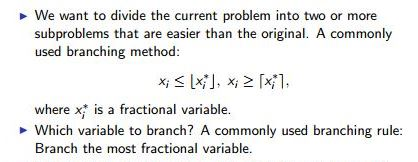
\includegraphics[width=1.1\linewidth]{NodeSelection1A}
		\end{figure}
	\end{frame}
	
	\begin{frame}
			\frametitle{Node Selection Strategies}
			\large
		\noindent \textbf{Floor and Ceiling Functions, and Fractional Components}
		\begin{itemize}
		\item The floor and ceiling functions map a real number to the largest previous or the smallest following integer, respectively. 
		\item More precisely, floor(x) = $\lfloor x\rfloor $ is the largest integer not greater than x and ceiling(x) =  $\lceil x \rceil$ is the smallest integer not less than x.
		\item The \textbf{fractional part}, is denoted by $\{x\}$ for real x and is defined by the formula
		\[\{x\} = x -\lfloor x\rfloor.\]
		\item For all x,
		$0\le\{x\}<1.\;$
		\end{itemize}
	\end{frame}
	%====================================================== %
	\begin{frame}
		\begin{figure}
\centering
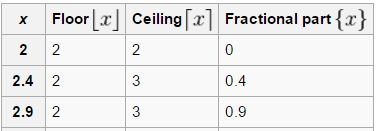
\includegraphics[width=1.0\linewidth]{floorceiling}

\end{figure}
\noindent The \textit{most fractional variable }is indicated by the number with the highest fractional part.
	\end{frame}
	%====================================================== %
	\begin{frame}
		\frametitle{Node Selection Strategies}
		\large
		\begin{figure}
			\centering
			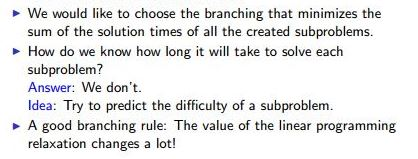
\includegraphics[width=1.1\linewidth]{NodeSelection1B}
		\end{figure}
	\end{frame}
	%====================================================== %
	\begin{frame}

		\begin{figure}
			\centering
			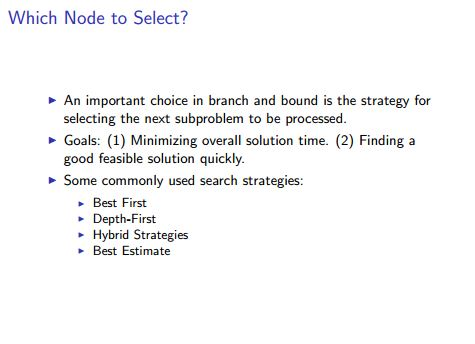
\includegraphics[width=1.2\linewidth]{NodeSelection2}
		\end{figure}
	\end{frame}
	%====================================================== %
	\begin{frame}

		\begin{figure}
			\centering
			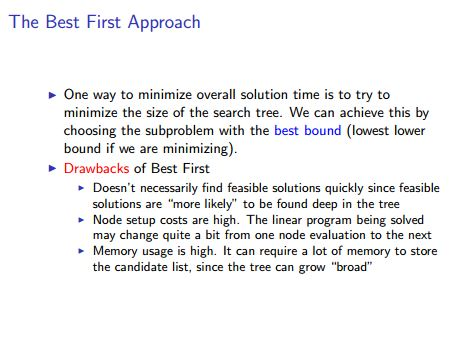
\includegraphics[width=1.15\linewidth]{NodeSelection3}
		\end{figure}
	\end{frame}
	%====================================================== %
	\begin{frame}
		\frametitle{Node Selection Strategies}
		\large
		\begin{figure}
			\centering
			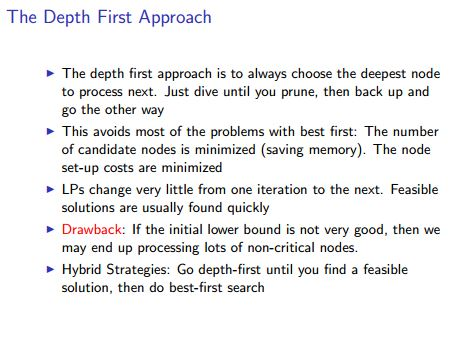
\includegraphics[width=1.1\linewidth]{NodeSelection4}
		\end{figure}
	\end{frame}
	%====================================================== %
	\begin{frame}
		\frametitle{Node Selection Strategies}
		\large
		\begin{figure}
			\centering
			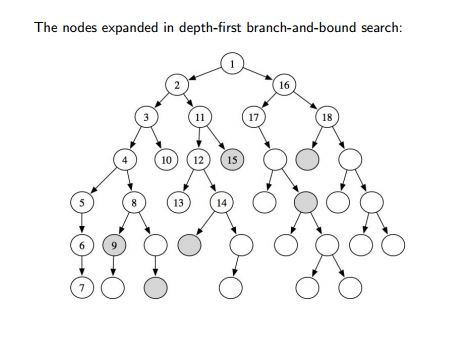
\includegraphics[width=1.1\linewidth]{NodeSelection5}
		\end{figure}
	\end{frame}
%====================================================== %
\begin{frame}
	\frametitle{Binary Integer Programming}
	\Large
	\noindent\textbf{Review}
	\begin{itemize}
		\item Be able to compare and contrast node selection strategies.
	\end{itemize}
\end{frame}
\end{document}